% !TeX encoding = UTF-8

% 载入 SJTUThesis 模版
\documentclass[type=course,lang=en]{sjtuthesis}
% 选项
%   type=[doctor|master|bachelor|course],     % 可选(默认:doctor),论文类型
%   zihao=[-4|5],                             % 可选(研究生默认:-4,本科默认:5),正文字号大小
%   lang=[zh|en],                             % 可选(默认:zh),论文的主要语言
%   review,                                   % 可选(默认:关闭),盲审模式
%   [twoside|oneside]                         % 可选(默认:twoside),单双页模式

% 论文基本配置,加载宏包等全局配置
% !TEX root = ./main.tex

\sjtusetup{
  %
  %******************************
  % 注意:
  %   1. 配置里面不要出现空行
  %   2. 不需要的配置信息可以删除
  %******************************
  %
  % 信息录入
  %
  info = {%
    %
    % 标题
    %
    title           = {Evolution and analysis of American music's genre},
    title*          = {Evolution and analysis of American music's genre},
    %
    % 标题页标题
    %   可使用“\\”命令手动控制换行
    %
    % display-title   = {上海交通大学学位论文\\ \LaTeX{} 模板示例文档},
    % display-title*  = {A Sample Document \\ for \LaTeX-based SJTU Thesis Template},
    %
    % 页眉标题
    %
    % running-title   = {示例文档},
    % running-title*  = {Sample Document},
    %
    % 关键词
    %
    keywords        = {上海交大, 饮水思源, 爱国荣校},
    keywords*       = {SJTU, master thesis, XeTeX/LaTeX template},
    %
    % 姓名
    %
    author          = {Basic Mathematical Statistics},
    author*         = {Mo Mo},
    %
    % 指导教师
    %
    supervisor      = {杨新宇\quad{}021020910058},
    supervisor*     = {Prof. Mou Mou},
    %
    % 副指导教师
    %
    % assisupervisor  = {某某教授},
    % assisupervisor* = {Prof. Uom Uom},
    %
    % 学号
    %
    id              = {秦子健\quad{}021020910010},
    %
    % 学位
    %   本科生不需要填写
    %
    degree          = {工学硕士},
    degree*         = {Master of Engineering},
    %
    % 专业
    %
    major           = {某某专业},
    major*          = {A Very Important Major},
    %
    % 所属院系
    %
    department      = {赵学涛\quad{}021010910018},
    department*     = {Depart of XXX},
    %
    % 课程名称
    %   仅课程论文适用
    %
    course          = {徐德全\quad{}021020910068},
    %
    % 答辩日期
    %   使用 ISO 格式 (yyyy-mm-dd);默认为当前时间
    %
    % date            = {2014-12-17},
    %
    % 资助基金
    %
    % fund  = {
    %           {国家 973 项目 (No. 2025CB000000)},
    %           {国家自然科学基金 (No. 81120250000)},
    %         },
    % fund* = {
    %           {National Basic Research Program of China (Grant No. 2025CB000000)},
    %           {National Natural Science Foundation of China (Grant No. 81120250000)},
    %         },
  },
  %
  % 风格设置
  %
  style = {%
    %
    % 本科论文页眉 logo 颜色 (red/blue/black)
    %
    % header-logo-color = black,
  },
  %
  % 名称设置
  %
  name = {
    % bib               = {References},
    % acknowledgements  = {谢\hspace{\ccwd}辞},
    % publications      = {攻读学位期间完成的论文},
  },
}

% 使用 BibLaTeX 处理参考文献
%   biblatex-gb7714-2015 常用选项
%     gbnamefmt=lowercase     姓名大小写由输入信息确定
%     gbpub=false             禁用出版信息缺失处理
\usepackage[backend=biber,style=gb7714-2015]{biblatex}
% 文献表字体
% \renewcommand{\bibfont}{\zihao{-5}}
% 文献表条目间的间距
\setlength{\bibitemsep}{0pt}
% 导入参考文献数据库
\addbibresource{bibdata/thesis.bib}

% 定义图片文件目录与扩展名
\graphicspath{{figures/}}
\DeclareGraphicsExtensions{.pdf,.eps,.png,.jpg,.jpeg}

% 确定浮动对象的位置,可以使用 [H],强制将浮动对象放到这里(可能效果很差)
% \usepackage{float}

% 固定宽度的表格
% \usepackage{tabularx}

% 使用三线表:toprule,midrule,bottomrule。
\usepackage{booktabs}

% 表格中支持跨行
\usepackage{multirow}

% 表格中数字按小数点对齐
\usepackage{dcolumn}
\newcolumntype{d}[1]{D{.}{.}{#1}}

% 使用长表格
\usepackage{longtable}

% 附带脚注的表格
\usepackage{threeparttable}

% 附带脚注的长表格
\usepackage{threeparttablex}

% 算法环境宏包
\usepackage[ruled,vlined,linesnumbered]{algorithm2e}
% \usepackage{algorithm, algorithmicx, algpseudocode}

% 代码环境宏包
\usepackage{listings}
\lstnewenvironment{codeblock}[1][]%
  {\lstset{style=lstStyleCode,#1}}{}

% 物理科学和技术中使用的数学符号,定义了 \qty 命令,与 siunitx 3.0 有冲突
% \usepackage{physics}

% 直立体数学符号
\newcommand{\dd}{\mathop{}\!\mathrm{d}}
\newcommand{\ee}{\mathrm{e}}
\newcommand{\ii}{\mathrm{i}}
\newcommand{\jj}{\mathrm{j}}

% 国际单位制宏包
\usepackage{siunitx}[=v2]

% 定理环境宏包
\usepackage{ntheorem}
% \usepackage{amsthm}

% 绘图宏包
\usepackage{tikz}
\usetikzlibrary{shapes.geometric, arrows}

% 一些文档中用到的 logo
\usepackage{hologo}
\newcommand{\XeTeX}{\hologo{XeTeX}}
\newcommand{\BibLaTeX}{\textsc{Bib}\LaTeX}

% 借用 ltxdoc 里面的几个命令方便写文档
\DeclareRobustCommand\cs[1]{\texttt{\char`\\#1}}
\providecommand\pkg[1]{{\sffamily#1}}

% 自定义命令

% E-mail
\newcommand{\email}[1]{\href{mailto:#1}{\texttt{#1}}}

% hyperref 宏包在最后调用
\usepackage{hyperref}

% 自动引用题注更正为中文
\def\equationautorefname{式}
\def\footnoteautorefname{脚注}
\def\itemautorefname{项}
\def\figureautorefname{图}
\def\tableautorefname{表}
\def\partautorefname{篇}
\def\appendixautorefname{附录}
\def\chapterautorefname{章}
\def\sectionautorefname{节}
\def\subsectionautorefname{小节}
\def\subsubsectionautorefname{小节}
\def\paragraphautorefname{段落}
\def\subparagraphautorefname{子段落}
\def\FancyVerbLineautorefname{行}
\def\theoremautorefname{定理}

%appendix 中代码正确显示
\usepackage{listings}
\usepackage{ctex}

% 用来设置附录中代码的样式

\lstset{
    basicstyle          =   \sffamily,          % 基本代码风格
    keywordstyle        =   \bfseries,          % 关键字风格
    commentstyle        =   \rmfamily\itshape,  % 注释的风格,斜体
    stringstyle         =   \ttfamily,  % 字符串风格
    flexiblecolumns,                % 别问为什么,加上这个
    numbers             =   left,   % 行号的位置在左边
    showspaces          =   false,  % 是否显示空格,显示了有点乱,所以不现实了
    numberstyle         =   \zihao{-5}\ttfamily,    % 行号的样式,小五号,tt等宽字体
    showstringspaces    =   false,
    captionpos          =   t,      % 这段代码的名字所呈现的位置,t指的是top上面
    frame               =   lrtb,   % 显示边框
}

\lstdefinestyle{Python}{
    language        =   Python, % 语言选Python
    basicstyle      =   \zihao{-5}\ttfamily,
    numberstyle     =   \zihao{-5}\ttfamily,
    keywordstyle    =   \color{blue},
    keywordstyle    =   [2] \color{teal},
    stringstyle     =   \color{magenta},
    commentstyle    =   \color{red}\ttfamily,
    breaklines      =   true,   % 自动换行,建议不要写太长的行
    columns         =   fixed,  % 如果不加这一句,字间距就不固定,很丑,必须加
    basewidth       =   0.5em,
}

\usepackage{amsmath}
% \usepackage{amssymb}

\begin{document}

%TC:ignore

% 标题页
\maketitle

% 原创性声明及使用授权书
%\copyrightpage
% 插入外置原创性声明及使用授权书
% \copyrightpage[scans/sample-copyright-old.pdf]

% 前置部分
\frontmatter

% 摘要
%% !TEX root = ../main.tex
\begin{}
\begin{abstract}
  中文摘要应该将学位论文的内容要点简短明了地表达出来,应该包含论文中的基本信息,
  体现科研工作的核心思想。摘要内容应涉及本项科研工作的目的和意义、研究方法、研究
  成果、结论及意义。注意突出学位论文中具有创新性的成果和新见解的部分。摘要中不宜
  使用公式、化学结构式、图表和非公知公用的符号和术语,不标注引用文献编号。硕士学
  位论文中文摘要字数为 500 字左右,博士学位论文中文摘要字数为 800 字左右。英文摘
  要内容应与中文摘要内容一致。

  摘要页的下方注明本文的关键词(4~6个)。
\end{abstract}

\begin{abstract*}
  Shanghai Jiao Tong University (SJTU) is a key university in China. SJTU was
  founded in 1896. It is one of the oldest universities in China. The University
  has nurtured large numbers of outstanding figures include JIANG Zemin, DING
  Guangen, QIAN Xuesen, Wu Wenjun, WANG An, etc.

  SJTU has beautiful campuses, Bao Zhaolong Library, Various laboratories. It
  has been actively involved in international academic exchange programs. It is
  the center of CERNet in east China region, through computer networks, SJTU has
  faster and closer connection with the world.
\end{abstract*}


% 目录
\tableofcontents
% 插图索引
%\listoffigures*
% 表格索引
%\listoftables*
% 算法索引
%\listofalgorithms*

% 符号对照表
%% !TEX root = ../main.tex

\begin{nomenclature*}
\label{chap:symb}

\begin{longtable}{rl}
  $\epsilon$  & 介电常数  \\  
  $\mu$       & 磁导率    \\
  $\epsilon$  & 介电常数  \\
  $\mu$       & 磁导率    \\
  $\epsilon$  & 介电常数  \\
  $\mu$       & 磁导率    \\
  $\epsilon$  & 介电常数  \\
  $\mu$       & 磁导率    \\
  $\epsilon$  & 介电常数  \\
  $\mu$       & 磁导率    \\
  $\epsilon$  & 介电常数  \\
  $\mu$       & 磁导率    \\
  $\epsilon$  & 介电常数  \\
  $\mu$       & 磁导率    \\
  $\epsilon$  & 介电常数  \\
  $\mu$       & 磁导率    \\
  $\epsilon$  & 介电常数  \\
  $\mu$       & 磁导率    \\
  $\epsilon$  & 介电常数  \\
  $\mu$       & 磁导率    \\
  $\epsilon$  & 介电常数  \\
  $\mu$       & 磁导率    \\
  $\epsilon$  & 介电常数  \\
  $\mu$       & 磁导率    \\
  $\epsilon$  & 介电常数  \\
  $\mu$       & 磁导率    \\
  $\epsilon$  & 介电常数  \\
  $\mu$       & 磁导率    \\
  $\epsilon$  & 介电常数  \\
  $\mu$       & 磁导率    \\
  $\epsilon$  & 介电常数  \\
  $\mu$       & 磁导率    \\
  $\epsilon$  & 介电常数  \\
  $\mu$       & 磁导率    \\
  $\epsilon$  & 介电常数  \\
  $\mu$       & 磁导率    \\
  $\epsilon$  & 介电常数  \\
  $\mu$       & 磁导率    \\
  $\epsilon$  & 介电常数  \\
  $\mu$       & 磁导率    \\
  $\epsilon$  & 介电常数  \\
  $\mu$       & 磁导率    \\
  $\epsilon$  & 介电常数  \\
  $\mu$       & 磁导率    \\
  $\epsilon$  & 介电常数  \\
  $\mu$       & 磁导率    \\
  $\epsilon$  & 介电常数  \\
  $\mu$       & 磁导率    \\
  $\epsilon$  & 介电常数  \\
  $\mu$       & 磁导率    \\
  $\epsilon$  & 介电常数  \\
  $\mu$       & 磁导率    \\
  $\epsilon$  & 介电常数  \\
  $\mu$       & 磁导率    \\
\end{longtable}

\end{nomenclature*}


%TC:endignore

% 主体部分
\mainmatter

% 正文内容
% !TEX root = ../main.tex

\chapter{杨新宇的部分}
% !TEX root = ../main.tex

\chapter{Influence Among Artists}

Some artists can list a dozen or more other artists who they say influenced their own musical work. It has also been suggested that influence can be measured by the degree of similarity between song characteristics, such as structure, rhythm, or lyrics. In this chapter, a directed network of influencers and followers is established according to ``influence\_data'' reported by the artists themselves, as well as the opinions of industry experts. In addition, the similarity of song characteristics among different artists is analysed to reflect the influence in another way. After a brief comparison between two influence networks, it may lead to some interesting results.

\section{A directed network of influencers and followers}

According to ``influence\_data'' and preceding entropy weight analysis, a directed network of influencers and followers can be established with each artist having a weight coefficient. For convenience of analysis and visualization, a sub-network including top 100 influential artists is built and plotted in Figure \ref{fig:influence}.\par

\begin{figure}
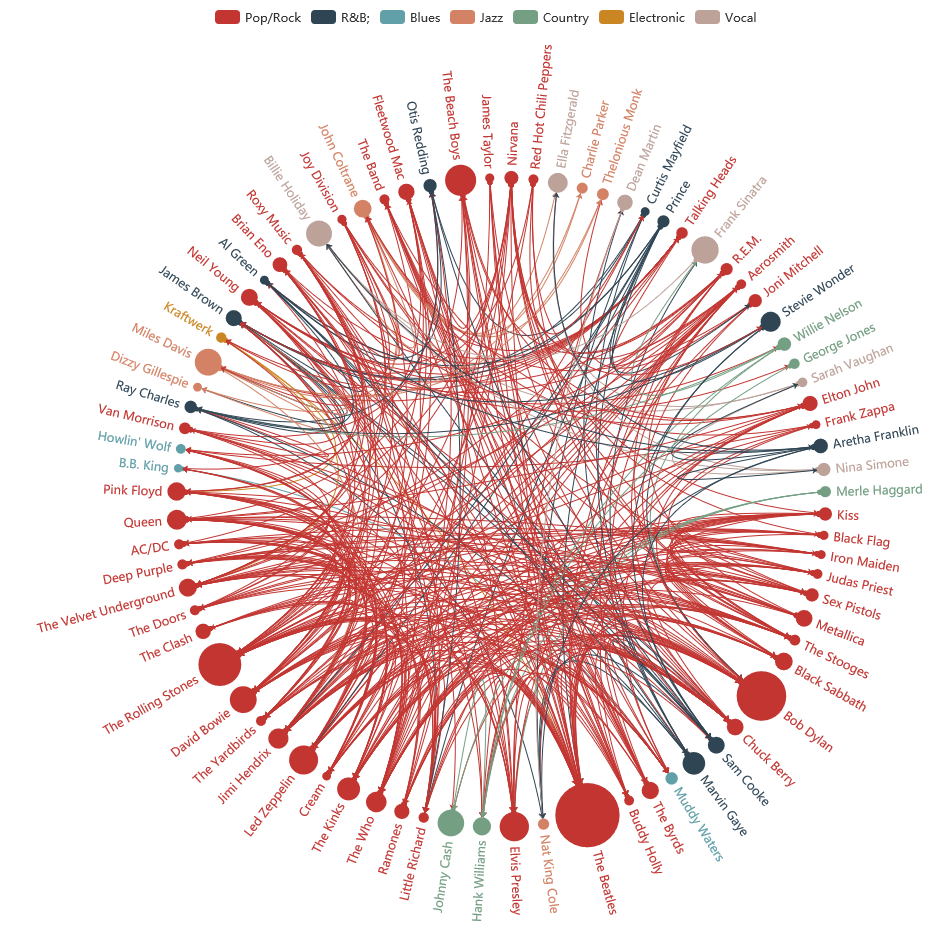
\includegraphics[width=1.25\textwidth]{figures/xdq/influence.png}
\setlength{\leftskip}{0pt plus 1fil minus \marginparwidth}
\setlength{\rightskip}{\leftskip}
\caption{A directed network of influencers and followers}
\label{fig:influence}
\end{figure}

In Figure \ref{fig:influence}, the size of a node represents the influence score of an artist and the direction of an arrow is from a follower to an influencer. It is clear that most of the top 100 artists are from genre Pop/Rock (in red colour). The Beatles, Bob Dylan, and The Rolling Stones come top 3 influential artists, which consists well with the previous analysis and the reality. The Beatles is regarded as the most influential band of all time; Bob Dylan is one of the greatest songwriters, and The Rolling Stone is one of the most famous rock bands. It is noticeable that in this network, the link between two artists has a specific direction, that is to say, one is the influencer while the other is influenced, which is different from similarity analysis. Moreover, an influencer can also be a follower, giving the fact that the most influential artist The Beatles is also influenced by ``The Band'' and Bob Dylan. This reveals the mutual influence of artists on each other.

\section{Similarity of music features among artists}

Similarity between song characteristics can also reflect musical influence among artists. To be clear, two artists sharing the similar music style would have a greater chance to be influenced by each other. This section is aimed to build another influence network based on similarity analysis.

\subsection{Euclidean similarity}

In $\mathbb{R}^n$, the Euclidean distance $||x-y||_2$ between two vectors $x = (x_1, x_2, ..., x_n)$ and $y = (y_1, y_2, ... , y_n)$ is always defined. It corresponds to the $L_2$-norm $||.||_2$ of the difference $x$--$y$ between the two vectors. It can be computed as:
\begin{equation}
\|x-y\|_{2}=\sqrt{\sum_{i=1}^{n}\left(x_{i}-y_{i}\right)^{2}}=\sqrt{\left(x_{1}-y_{1}\right)^{2}+\left(x_{2}-y_{2}\right)^{2}+\ldots+\left(x_{n}-y_{n}\right)^{2}}
\end{equation}
Here, PC1--PC7 are 7 major components reflecting the music style, so the Euclidean distance between two artists' music characteristics is:
\begin{equation}
dist_{i,j}=\sqrt{\sum_{k=1}^{7}\left(P C_{k}^{i}-P C_{k}^{j}\right)^{2}}
\end{equation}
In order to get a similarity coefficient ranging from 0 to 1, we define Euclidean similarity as:
\begin{equation}
Sim_{L2}^{i,j}=\frac{1}{dist_{i, j}+1}
\end{equation}

\subsection{Cosine similarity}

In data analysis, cosine similarity is a measure of similarity between two sequences of numbers. For defining it, the sequences are viewed as vectors in an inner product space, and the cosine similarity is defined as the cosine of the angle between them, that is, the dot product of the vectors divided by the product of their lengths, as shown in Equation \eqref{cosine}. It follows that the cosine similarity does not depend on the magnitudes of the vectors, but only on their angle. The cosine similarity always belongs to the interval [-1,1]. 

\begin{equation}
Sim_{cos}^{i, j}=\frac{\sum_{k=1}^{7} P C_{k}^{i} P C_{k}^{j}}{\sqrt{\sum_{k=1}^{7}\left(P C_{k}^{i}\right)^{7}} \sqrt{\sum_{k=1}^{7}\left(P C_{k}^{j}\right)^{2}}}
\label{cosine}
\end{equation}

\subsection{Similarity of music characteristics among artists}

The data set ``data\_by\_artis'' provides us with more than 10 musical features of each artist, such as danceability, tempo, loudness and etc. After PCA and entropy weight analysis, we select 100 most influential artists to measure their similarities among each other. Euclidean similarity could reflect the distance between 2 vectors in the space, while some problems may occur when two vectors are close to the original point but in totally different directions. Cosine similarity is useful to reveal the similarity in directions, neglecting the information of length. It would be more reasonable to consider both Euclidean similarity and cosine similarity in this case. We define that two artists share the similar music style (have a potential to influence each other), when:
\begin {equation}
Sim_{cos}^{i, j}>0.7 \qquad \text{and} \qquad Sim_{L2}^{i,j}>0.7
\end{equation}

Under such criterion, a new influence network is established based on similarity analysis, as shown in Figure \ref{fig:similarity}.

\begin{figure}
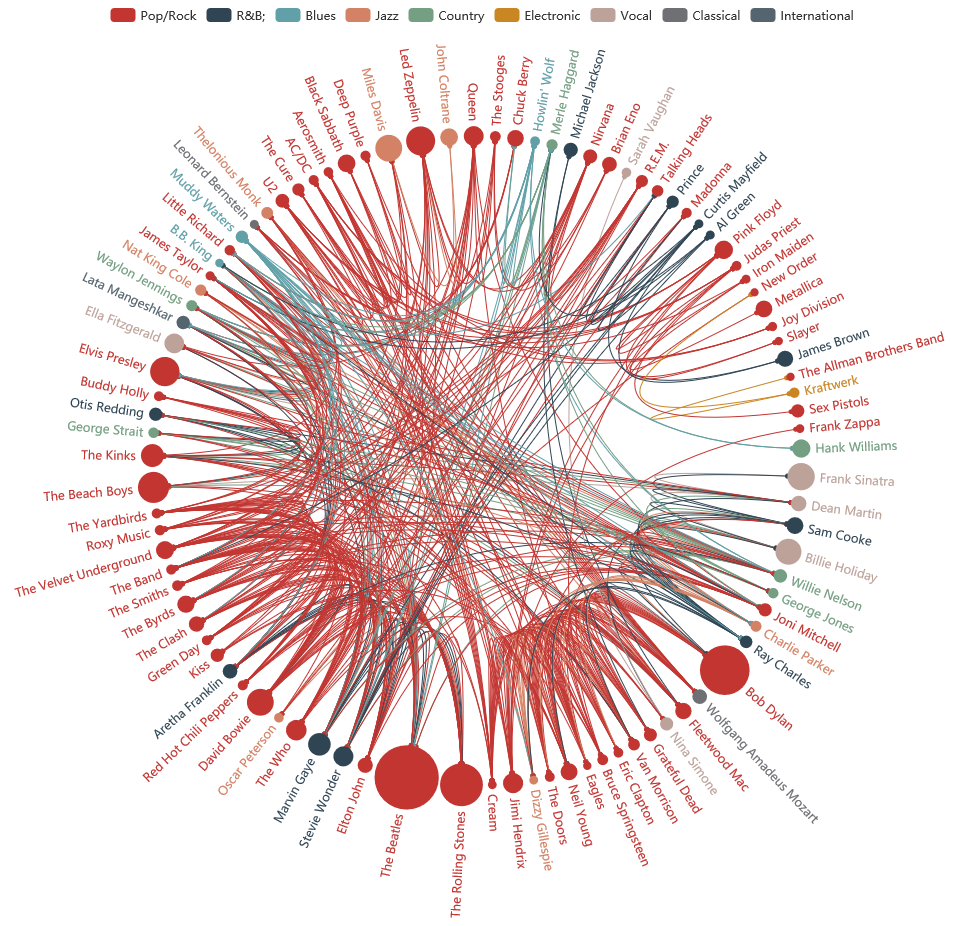
\includegraphics[width=1.25\textwidth]{figures/xdq/similarity.png}
\setlength{\leftskip}{0pt plus 1fil minus \marginparwidth}
\setlength{\rightskip}{\leftskip}
\caption{An influence network based on musical similarity}
\label{fig:similarity}
\end{figure}

\section{A comparison between two influence networks}

So far, two influence networks have been obtained. The first directed one (Figure \ref{fig:influence}) is reported by the artists themselves, as well as the opinions of industry experts. The latter one without arrows is established by the degree of similarity between song characteristics, such as structure, rhythm, or lyrics. We are curious about the difference between them, and hopefully we expect to find some interesting information. 

Generally speaking, most artists are mainly influenced by artists within the same genre as reported in the first network, while more between-genre-influence relationships are witnessed in the second network. This phenomenon is contributed to the subjectivity involved in the interviews or comments. Artists tend to claim they follow the famous musicians in the genre they belong to. In addition, industry experts often start from a professional manner to make judgements, that is to say, the genre barrier cannot be overlooked in this scenario.

To be specific, each artist has a list of ``nominal'' (self-claimed) followers and a list of potential professional fans (based on musical similarity). These two lists may overlap to some extend, indicating that a ``double-checked'' strong bond among artists exists.

For simplicity and convenience, the influence data of the famous artist Bob Dylan is taken as an example for analysis. Two mini influence networks related to Bob Dylan are shown in Figure \ref{fig:bob1} and \ref{fig:bob2}.

\begin{figure}[htbp]
    \setlength{\leftskip}{0pt plus 1fil minus \marginparwidth}
    \setlength{\rightskip}{\leftskip}
    \begin{subfigure}{0.5\linewidth}
        \centering
        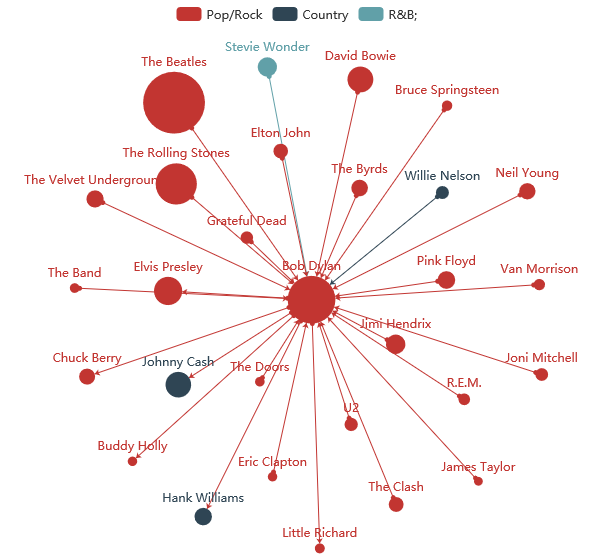
\includegraphics[width=\textwidth]{figures/xdq/BOB1.png}
        \caption{reported by artists \& experts}
        \label{fig:bob1}
    \end{subfigure}
    \begin{subfigure}{0.5\linewidth}
        \centering
        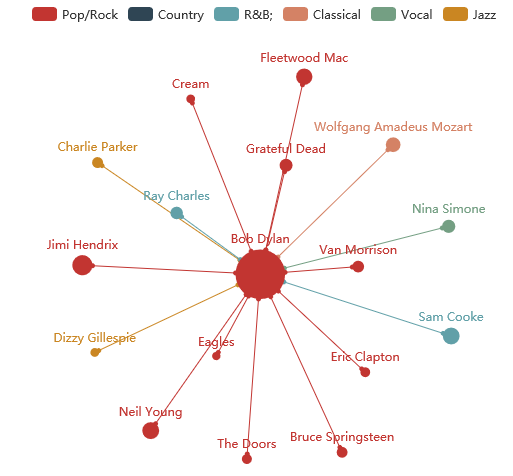
\includegraphics[width=\textwidth]{figures/xdq/BOB2.png}
        \caption{computed from similarity analysis}
        \label{fig:bob2}
    \end{subfigure}
    \caption{Bob Dylan influence networks}
\end{figure}


% \begin{figure}
% 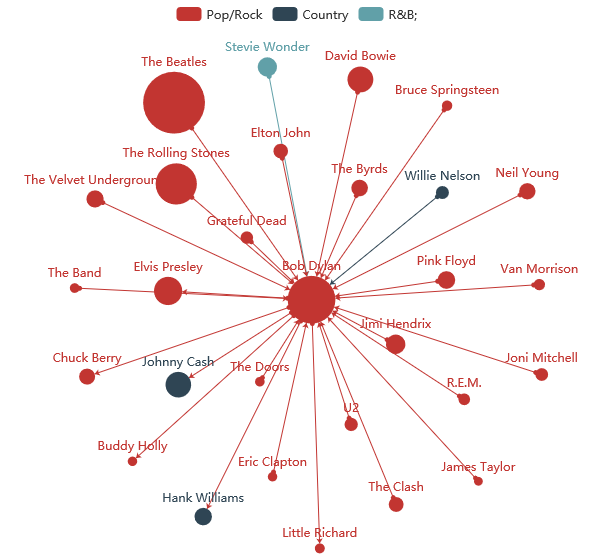
\includegraphics[width=0.5\textwidth]{figures/xdq/BOB1.png}
% \centering
% \caption{Bob Dylan influence network 1: reported by artists}
% \label{fig:bob1}
% \end{figure}

% \begin{figure}
% 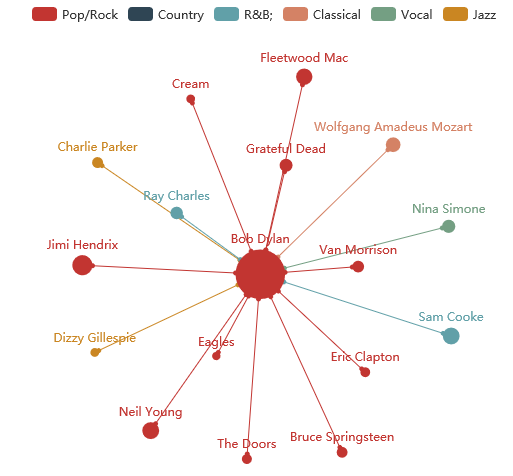
\includegraphics[width=0.5\textwidth]{figures/xdq/BOB2.png}
% \centering
% \caption{Bob Dylan influence network 2: from similarity analysis}
% \label{fig:bob2}
% \end{figure}

The left figure shows the artists that have influenced on or been influenced by Bob Dylan according to data reported by artists \& experts. The right one illustrates the artists sharing similar music features with Bob Dylan. 7 artists appear in both networks, indicating a strong influence --- not only orally judged by person, but also reflected in their musical works. They are: Grateful Dead,Van Morrison, Eric Clapton, Bruce Springsteen, Neil Young, The Doors and Jimi Hendrix. We also checked whether some self-claimed followers have a very different music style with their influencer, and the result shows that no one does.



% \begin{enumerate}
%     \item 谁才是Bob Dylan的忠实拥趸?
%     \begin{enumerate}
%         \item Grateful Dead
%         \item Van Morrison
%         \item Eric Clapton
%         \item Bruce Springsteen
%         \item Neil Young
%         \item The Doors
%         \item Jimi Hendrix
%     \end{enumerate}
%     \item 谁又与Bob Dylan的曲风大相径庭?
%      \begin{enumerate}
%         \item 《震惊,潮水退去,竟是他在裸泳!!!》
%         \item 《你为什么接受采访,你是不是有什么不可告人的目的?》
%         \item 《谁指使你这么说的?》
%         \item to be continued 2022.05.25
%     \end{enumerate}
% \end{enumerate}


% % test
% \begin{figure}
%     \centering
%     
% 定义流程图节点
\tikzstyle{startstop} = [
  rectangle,
  rounded corners,
  minimum width=2cm,
  minimum height=1cm,
  text centered,
  draw=black
]
\tikzstyle{io} = [
  trapezium,
  trapezium left angle=75,
  trapezium right angle=105,
  minimum width=1cm,
  minimum height=1cm,
  text centered,
  draw=black
]
\tikzstyle{process} = [
  rectangle,
  minimum width=2cm,
  minimum height=1cm,
  text centered,
  draw=black
]
\tikzstyle{decision} = [
  diamond,
  minimum width=2cm,
  minimum height=1cm,
  text centered,
  draw=black]
\tikzstyle{arrow} = [thick, ->, >=stealth]

\begin{tikzpicture}[node distance=2cm]
  % 设置节点
  \node (pic) [startstop] {待测图片};
  \node (bg) [io, below of=pic] {读取背景};
  \node (pair) [process, below of=bg] {匹配特征点对};
  \node (threshold) [decision, below of=pair, yshift=-0.5cm] {多于阈值};
  \node (clear) [decision, right of=threshold, xshift=3cm] {清晰?};
  \node (capture) [process, right of=pair, xshift=3cm, yshift=0.5cm] {重采};
  \node (matrix_p) [process, below of=threshold, yshift=-0.8cm] {透视变换矩阵};
  \node (matrix_a) [process, right of=matrix_p, xshift=3cm] {仿射变换矩阵};
  \node (reg) [process, below of=matrix_p] {图像修正};
  \node (return) [startstop, below of=reg] {配准结果};
    
  % 连接节点
  \draw [arrow](pic) -- (bg);
  \draw [arrow](bg) -- (pair);
  \draw [arrow](pair) -- (threshold);

  \draw [arrow](threshold) -- node[anchor=south] {否} (clear);

  \draw [arrow](clear) -- node[anchor=west] {否} (capture);
  \draw [arrow](capture) |- (pic);
  \draw [arrow](clear) -- node[anchor=west] {是} (matrix_a);
  \draw [arrow](matrix_a) |- (reg);

  \draw [arrow](threshold) -- node[anchor=east] {是} (matrix_p);
  \draw [arrow](matrix_p) -- (reg);
  \draw [arrow](reg) -- (return);
\end{tikzpicture}

%     \caption{Caption}
%     \label{fig:my_label}
% \end{figure}

% !TEX root = ../main.tex

\chapter{Cluster Analysis}

% 这是中文
% 在原始的数据中,我们将艺术家划分了流派,但是一个人创作的音乐可能有着不同的风格,因此我们要对音乐的数据进行聚类分析,并对其进行分类。在聚类的方法上,选用了K-means聚类和层次聚类两种方法,并对聚类的结果进行了评估。


\section{Data Preprocessing}
% 在进行聚类分析之前,需要对数据进行预处理。
\subsection{Entropy Weight Process}
%首先在数据的选择上,由于原始数据有将近十万首歌曲的数据,我们只需要对有一定影响力的艺术家创作的歌曲进行分析,因此选择由熵权法确定的影响力前100位的艺术家创作的歌曲,共计2万多首。 

\subsection{PCA Dimensionality Reduction}
\section{Cluster Method}
% 主要使用K-means和层次聚类的方法

\subsection{K-means Cluster}
% 聚类方法介绍

\subsection{Hierarchical Cluster}

\section{Cluster Evaluation}

\subsection{Within-cluster Sum of Squared Errors(SSE)}
% 簇内误差平方和

\subsection{Silhouette Analysis}
% 轮廓系数silhouette coefficient

\section{Visualization of Clusters}
% !TEX root = ../main.tex

\chapter{Machine Learning}
We apply PNN(Probabilistic Neural Network) for machine learning.PNN can be regarded as a Radial Basis Neutral Network,it’s based on the Radial Basis Function(RBF) network and involved Density function estimation and Bayesian decision theory.Under most conditions,PNN can realize the discriminant boundary asymptotically approaching the Bayesian optimal decision surface.
\section{Neural network structure of PNN}
PNN is consist of input layer,Radial Basis Layer(hidden layer) and competitive layer(output layer),which is shown in ~\ref{fig:structure of PNN}.The first layer is the input layer,it’s used to receive training sample and transfer data to hidden layer.The hidden layer is Radial basis layer,it receives samples form the input layer and return a scalar which depends on the Euclidean distance to the center vector.the scalars are transferred to the output layer,which is a competition layer,which can output the scalar that satisfy the competition requirement.During the training process,we are able to achieve the center vector and variance of each class.In the later testing process,through calculating the Euclidean distance from the sample to each center vector and transform into the probability of decision based on Bayesian optimal decision.
\begin{figure}
    \centering
    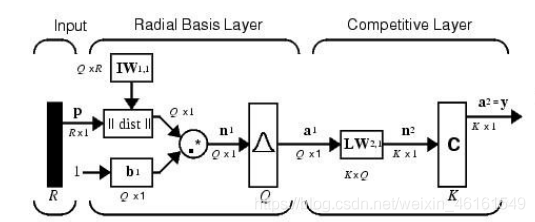
\includegraphics[width=0.9\textwidth]{figures/PNN neural network.png}
    \caption{structure of PNN}
    \label{fig:structure of PNN}
\end{figure}
\subsection{Radial Basis Function(RBF)}
The main idea of the RBF layer is using the RBF as the basis of the latent space,this allows the input vector to be directly mapped to the latent space without connecting through weights.When the center point of the RBF is determined after the training process,the mapping relationship is also determined.Among them, the role of the hidden layer is to map the vector from the low-dimensional \verb+p+ to the high-dimensional \verb+h+, so that the low-dimensional linear inseparability can become linearly separable to the high-dimensional,which is the main idea of the kernel function. In this way, the mapping of the network from input to output is nonlinear, while the network output is linear with respect to adjustable parameters. The weights of the network can be directly solved by the linear equation system, which greatly speeds up the learning speed and avoids the local minimal problem.
the activative function of the raidal basis neural network can be written as
\begin{equation}
\operatorname\\{R}({x}_{p}-{c}_{i})=
\\exp{(-\frac{1}{2\,\sigma_i^2} \Vert {x}_{p}-{c}_{i}\Vert_2^2})
\end{equation}
As we can see,if the sample vector ${x}_{p}$ is closed to the center vector ${c}_{i}$,$R$ would be more closed to $1$,based on this,we are able to build the connction from $R$ to the probability of decision through Bayesian optimal decision.
\subsection{Bayesian optimal decision theory}
The competition layer(output layer)is based on the Bayesian optimal decision theory.
for a typicalbinary classification problem: $c=c_1$ or $c=c_2$.Prior probability can be written as
\begin{equation}
{h}_{1}=\\{p}({c}_{1}),{h}_{2}=\\{p}({c}_{2}),{h}_{1}+{h}_{2}=1
\end{equation}
for any input vector $x = [x_1,\ldots,x_n]$,the classification criterion are shown below:
\begin{equation}
    {c}=
    \begin{cases}
    c_1,p(c_1|x)>p(c_2|{x}),\\
    c_2,otherwise
    \end{cases}
\end{equation}
${p}({c}_{i}|{x})$ is defined as when $x$ happens,the posterior probability of $c_i$.According to the Bayesian function.the posterior probability equals to 
\begin{equation}
    p(c_i|x)=\frac{ p(c_i)p(x|c_i)}{ p(x)}
\end{equation}
during the decision making process,the classification criterion should be the posterior probability.In practical situation,cost of misclassification are need to be considered.The cost of missclassify type 1 sample into type 2 and missclassify type2 sample into type1 are sometimes different.Therefore,the classification are needed to be adujusted.Define event $\alpha_{1}$ is classify the input vector into type $c_i$,the cost of misclassification is $\lambda_{ij}$.So the expectation cost of apply event $\alpha_{1}$ is
\begin{equation}
    \\R(\alpha_i|\\x)=\sum_{j=1}^{N} \lambda_{ij}\\p(c_i|\\x)
\end{equation}
Assume that the cost of correctly classification is $0$,the expectation cost of event $\alpha_{1}$ is
\begin{equation}
     \\R(\alpha_i|\\x)= \lambda_{12}\\p(c_2|\\x)
\end{equation}
The Bayesian theorem turns into
\begin{equation}
    {c}=
    \begin{cases}
    c_1,R(c_1|x)<R(c_2|{x}),\\
    c_2,otherwise
    \end{cases}
\end{equation}
However,in the project,we assume that the cost of missclassification are equals,so the classification only depends on the probability of events.
\section{Summary of implementing PNN}
Firstly,based on the label of the training set,we are able to attain the center vector $u_j$ and variance $\sigma_j$ of class $j$.
\begin{equation}
    u_j=min{\sum_i}\Vert x_{ij}-u_j\Vert_2^2\\
\end{equation}
\begin{equation}
    \sigma_j=\sqrt{\frac{1}{N}\sum_{i=1}^{N}\Vert x_{ij}-u_j\Vert_2^2}
\end{equation}
where $K$ is the number of class $j$.
\par
Secondly,for each new sample $x_i$ in the testing layer,we apply the RBF to transform the Euclidean distance between $x_i$ and center vector of each classes $u_j$ into a real number $\phi_{ij}$ ranging from $0$ to $1$.then,we normalize $\phi_{ij}$ and regard it as the probability of classification.
\begin{equation}
    \phi_{ij}=\\exp{(-\frac{1}{2\,\sigma_j^2} \Vert {x}_{ij}-{u}_{j}\Vert_2^2})
\end{equation}
\begin{equation}
    p_{ij}=\frac{\phi_{ij}}{\sum_{j}\phi_{ij}}
\end{equation}
which means the probability of classifying sample $x_i$ into class $j$.
\par
Lately,we apply the Bayesian optimal theorem as the decision criterion and output the result.
\par
In order to clearify and simplify the result,we only select several singer's songs as the entire sample.randomly choose $80\%$ of the entire sample(16891) as the training set while the rest $20\%$(4222) is the testing set.the Accuracy of the training set and the testing set are around $97\%$(shown in \ref{fig:estimationresult}),which indicates the effectiveness and accuracy of the PNN to the problem.
\begin{figure}[b]
    \centering
    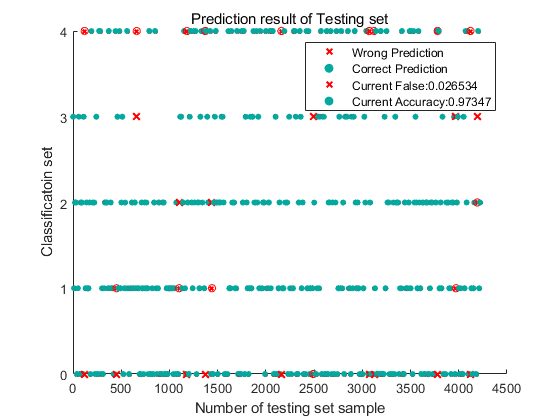
\includegraphics[width=0.85\textwidth]{figures/zxt/estimationresult.png}
    \caption{Prediction result of Testing Set}
    \label{fig:estimationresult}
\end{figure}

%TC:ignore

% 参考文献
%\printbibliography[heading=bibintoc]

% 附录
\appendix

% 附录中图表不加入索引
\captionsetup{list=no}

% 附录内容
%% !TEX root = ../main.tex

\chapter{Maxwell Equations}

选择二维情况,有如下的偏振矢量:
\begin{subequations}
  \begin{align}
    {\bf E} &= E_z(r, \theta) \hat{\bf z}, \\
    {\bf H} &= H_r(r, \theta) \hat{\bf r} + H_\theta(r, \theta) \hat{\bm\theta}.
  \end{align}
\end{subequations}
对上式求旋度:
\begin{subequations}
  \begin{align}
    \nabla \times {\bf E} &= \frac{1}{r} \frac{\partial E_z}{\partial\theta}
      \hat{\bf r} - \frac{\partial E_z}{\partial r} \hat{\bm\theta}, \\
    \nabla \times {\bf H} &= \left[\frac{1}{r} \frac{\partial}{\partial r}
      (r H_\theta) - \frac{1}{r} \frac{\partial H_r}{\partial\theta} \right]
      \hat{\bf z}.
  \end{align}
\end{subequations}
因为在柱坐标系下,$\overline{\overline\mu}$ 是对角的,所以 Maxwell 方程组中电场
$\bf E$ 的旋度:
\begin{subequations}
  \begin{align}
    & \nabla \times {\bf E} = \ii \omega {\bf B}, \\
    & \frac{1}{r} \frac{\partial E_z}{\partial\theta} \hat{\bf r} -
      \frac{\partial E_z}{\partial r}\hat{\bm\theta} = \ii \omega \mu_r H_r
      \hat{\bf r} + \ii \omega \mu_\theta H_\theta \hat{\bm\theta}.
  \end{align}
\end{subequations}
所以 $\bf H$ 的各个分量可以写为:
\begin{subequations}
  \begin{align}
    H_r &= \frac{1}{\ii \omega \mu_r} \frac{1}{r}
      \frac{\partial E_z}{\partial\theta}, \\
    H_\theta &= -\frac{1}{\ii \omega \mu_\theta}
      \frac{\partial E_z}{\partial r}.
  \end{align}
\end{subequations}
同样地,在柱坐标系下,$\overline{\overline\epsilon}$ 是对角的,所以 Maxwell 方程
组中磁场 $\bf H$ 的旋度:
\begin{subequations}
  \begin{align}
    & \nabla \times {\bf H} = -\ii \omega {\bf D}, \\
    & \left[\frac{1}{r} \frac{\partial}{\partial r}(r H_\theta) - \frac{1}{r}
      \frac{\partial H_r}{\partial\theta} \right] \hat{\bf z} = -\ii \omega
      {\overline{\overline\epsilon}} {\bf E} = -\ii \omega \epsilon_z E_z
      \hat{\bf z}, \\
    & \frac{1}{r} \frac{\partial}{\partial r}(r H_\theta) - \frac{1}{r}
      \frac{\partial H_r}{\partial\theta} = -\ii \omega \epsilon_z E_z.
  \end{align}
\end{subequations}
由此我们可以得到关于 $E_z$ 的波函数方程:
\begin{equation}
  \frac{1}{\mu_\theta \epsilon_z} \frac{1}{r} \frac{\partial}{\partial r}
  \left(r \frac{\partial E_z}{\partial r} \right) + \frac{1}{\mu_r \epsilon_z}
  \frac{1}{r^2} \frac{\partial^2E_z}{\partial\theta^2} +\omega^2 E_z = 0.
\end{equation}

% %!TEX root = ../main.tex

\chapter{绘制流程图}

图~\ref{fig:flow_chart} 是一张流程图示意。使用 \pkg{tikz} 环境,搭配四种预定义节
点(\verb+startstop+、\verb+process+、\verb+decision+和\verb+io+),可以容易地绘
制出流程图。

\begin{figure}[!htp]
  \centering
  \resizebox{6cm}{!}{
% 定义流程图节点
\tikzstyle{startstop} = [
  rectangle,
  rounded corners,
  minimum width=2cm,
  minimum height=1cm,
  text centered,
  draw=black
]
\tikzstyle{io} = [
  trapezium,
  trapezium left angle=75,
  trapezium right angle=105,
  minimum width=1cm,
  minimum height=1cm,
  text centered,
  draw=black
]
\tikzstyle{process} = [
  rectangle,
  minimum width=2cm,
  minimum height=1cm,
  text centered,
  draw=black
]
\tikzstyle{decision} = [
  diamond,
  minimum width=2cm,
  minimum height=1cm,
  text centered,
  draw=black]
\tikzstyle{arrow} = [thick, ->, >=stealth]

\begin{tikzpicture}[node distance=2cm]
  % 设置节点
  \node (pic) [startstop] {待测图片};
  \node (bg) [io, below of=pic] {读取背景};
  \node (pair) [process, below of=bg] {匹配特征点对};
  \node (threshold) [decision, below of=pair, yshift=-0.5cm] {多于阈值};
  \node (clear) [decision, right of=threshold, xshift=3cm] {清晰?};
  \node (capture) [process, right of=pair, xshift=3cm, yshift=0.5cm] {重采};
  \node (matrix_p) [process, below of=threshold, yshift=-0.8cm] {透视变换矩阵};
  \node (matrix_a) [process, right of=matrix_p, xshift=3cm] {仿射变换矩阵};
  \node (reg) [process, below of=matrix_p] {图像修正};
  \node (return) [startstop, below of=reg] {配准结果};
    
  % 连接节点
  \draw [arrow](pic) -- (bg);
  \draw [arrow](bg) -- (pair);
  \draw [arrow](pair) -- (threshold);

  \draw [arrow](threshold) -- node[anchor=south] {否} (clear);

  \draw [arrow](clear) -- node[anchor=west] {否} (capture);
  \draw [arrow](capture) |- (pic);
  \draw [arrow](clear) -- node[anchor=west] {是} (matrix_a);
  \draw [arrow](matrix_a) |- (reg);

  \draw [arrow](threshold) -- node[anchor=east] {是} (matrix_p);
  \draw [arrow](matrix_p) -- (reg);
  \draw [arrow](reg) -- (return);
\end{tikzpicture}
}
  \bicaption{绘制流程图效果}{Flow chart}
  \label{fig:flow_chart}
\end{figure}


% 结尾部分
\backmatter

% 用于盲审的论文需隐去致谢、发表论文、科研成果、简历

% 致谢
%% !TEX root = ../main.tex

\begin{acknowledgements}
  感谢那位最先制作出博士学位论文 \LaTeX 模板的交大物理系同学!

  感谢 William Wang 同学对模板移植做出的巨大贡献!

  感谢 \href{https://github.com/weijianwen}{@weijianwen} 学长一直以来的开发和维
  护工作!

  感谢 \href{https://github.com/sjtug}{@sjtug} 以及
   \href{https://github.com/dyweb}{@dyweb} 对 0.9.5 之后版本的开发和维护工作!

  感谢所有为模板贡献过代码的同学们, 以及所有测试和使用模板的各位同学!

  感谢 \LaTeX 和 \href{https://github.com/sjtug/SJTUThesis}{\sjtuthesis},帮我节
  省了不少时间。
\end{acknowledgements}


% 发表论文及科研成果
% 盲审论文中,发表论文及科研成果等仅以第几作者注明即可,不要出现作者或他人姓名
%% !TEX root = ../main.tex

\begin{achievements}

\subsection*{学术论文}

\begin{bibliolist}{00}
  \item Chen H, Chan C~T. Acoustic cloaking in three dimensions using acoustic metamaterials[J]. Applied Physics Letters, 2007, 91:183518.
  \item Chen H, Wu B~I, Zhang B, et al. Electromagnetic Wave Interactions with a Metamaterial Cloak[J]. Physical Review Letters, 2007, 99(6):63903.
\end{bibliolist}

\begin{bibliolist*}{00}
  \item 第一作者. 中文核心期刊论文, 2007.
  \item 第一作者. EI 国际会议论文, 2006.
\end{bibliolist*}

\subsection*{专利}

\begin{bibliolist}{00}
  \item 第一发明人,“永动机”,专利申请号202510149890.0
\end{bibliolist}

\begin{bibliolist*}{00}
  \item 第一发明人,“永动机”,专利申请号XXXXXXXXXXXX.X
\end{bibliolist*}

\end{achievements}


% 简历
%% !TEX root = ../main.tex

\begin{resume}
  \subsection*{基本情况}
    某某,yyyy 年 mm 月生于 xxxx。

  \subsection*{教育背景}
  \begin{itemize}
    \item yyyy 年 mm 月至今,上海交通大学,博士研究生,xx 专业
    \item yyyy 年 mm 月至 yyyy 年 mm 月,上海交通大学,硕士研究生,xx 专业
    \item yyyy 年 mm 月至 yyyy 年 mm 月,上海交通大学,本科,xx 专业
  \end{itemize}

  \subsection*{研究兴趣}
    \LaTeX{} 排版

  \subsection*{联系方式}
  \begin{itemize}
    \item 地址: 上海市闵行区东川路 800 号,200240
    \item E-mail: \email{xxx@sjtu.edu.cn}
  \end{itemize}
\end{resume}


% 学士学位论文要求在最后有一个大摘要,单独编页码
%% !TEX root = ../main.tex

\begin{digest}
  An imperial edict issued in 1896 by Emperor Guangxu, established Nanyang
  Public School in Shanghai. The normal school, school of foreign studies,
  middle school and a high school were established. Sheng Xuanhuai, the person
  responsible for proposing the idea to the emperor, became the first president
  and is regarded as the founder of the university.

  During the 1930s, the university gained a reputation of nurturing top
  engineers. After the foundation of People's Republic, some faculties were
  transferred to other universities. A significant amount of its faculty were
  sent in 1956, by the national government, to Xi'an to help build up Xi'an Jiao
  Tong University in western China. Afterwards, the school was officially
  renamed Shanghai Jiao Tong University.

  Since the reform and opening up policy in China, SJTU has taken the lead in
  management reform of institutions for higher education, regaining its vigor
  and vitality with an unprecedented momentum of growth. SJTU includes five
  beautiful campuses, Xuhui, Minhang, Luwan Qibao, and Fahua, taking up an area
  of about 3,225,833 m2. A number of disciplines have been advancing towards the
  top echelon internationally, and a batch of burgeoning branches of learning
  have taken an important position domestically.

  Today SJTU has 31 schools (departments), 63 undergraduate programs, 250
  masters-degree programs, 203 Ph.D. programs, 28 post-doctorate programs, and
  11 state key laboratories and national engineering research centers.

  SJTU boasts a large number of famous scientists and professors, including 35
  academics of the Academy of Sciences and Academy of Engineering, 95 accredited
  professors and chair professors of the "Cheung Kong Scholars Program" and more
  than 2,000 professors and associate professors.

  Its total enrollment of students amounts to 35,929, of which 1,564 are
  international students. There are 16,802 undergraduates, and 17,563 masters
  and Ph.D. candidates. After more than a century of operation, Jiao Tong
  University has inherited the old tradition of "high starting points, solid
  foundation, strict requirements and extensive practice." Students from SJTU
  have won top prizes in various competitions, including ACM International
  Collegiate Programming Contest, International Mathematical Contest in Modeling
  and Electronics Design Contests. Famous alumni include Jiang Zemin, Lu Dingyi,
  Ding Guangen, Wang Daohan, Qian Xuesen, Wu Wenjun, Zou Taofen, Mao Yisheng,
  Cai Er, Huang Yanpei, Shao Lizi, Wang An and many more. More than 200 of the
  academics of the Chinese Academy of Sciences and Chinese Academy of
  Engineering are alumni of Jiao Tong University.
\end{digest}


%TC:endignore

\end{document}
